An electron can be misidentified as a photon if the association of tracks or track seeds to the ECAL supercluster fails in the reconstruction step.
The production of a single \PW\ boson decaying to an electron and a neutrino is a high-rate process, and it mimicks the photon plus \met\ signature if the electron is misidentified.
We estimate the rate of misidentified electrons in the signal region by reweighting an electon proxy control sample by the ratio of the probability of an electron missing a pixel seed to the probability of an electron having a pixel seed. 
This procedure is shown in Figure~\ref{fig:efake_diagram}.

\begin{figure}[htbp]
  \centering
  \resizebox{0.95\textwidth}{!}{
    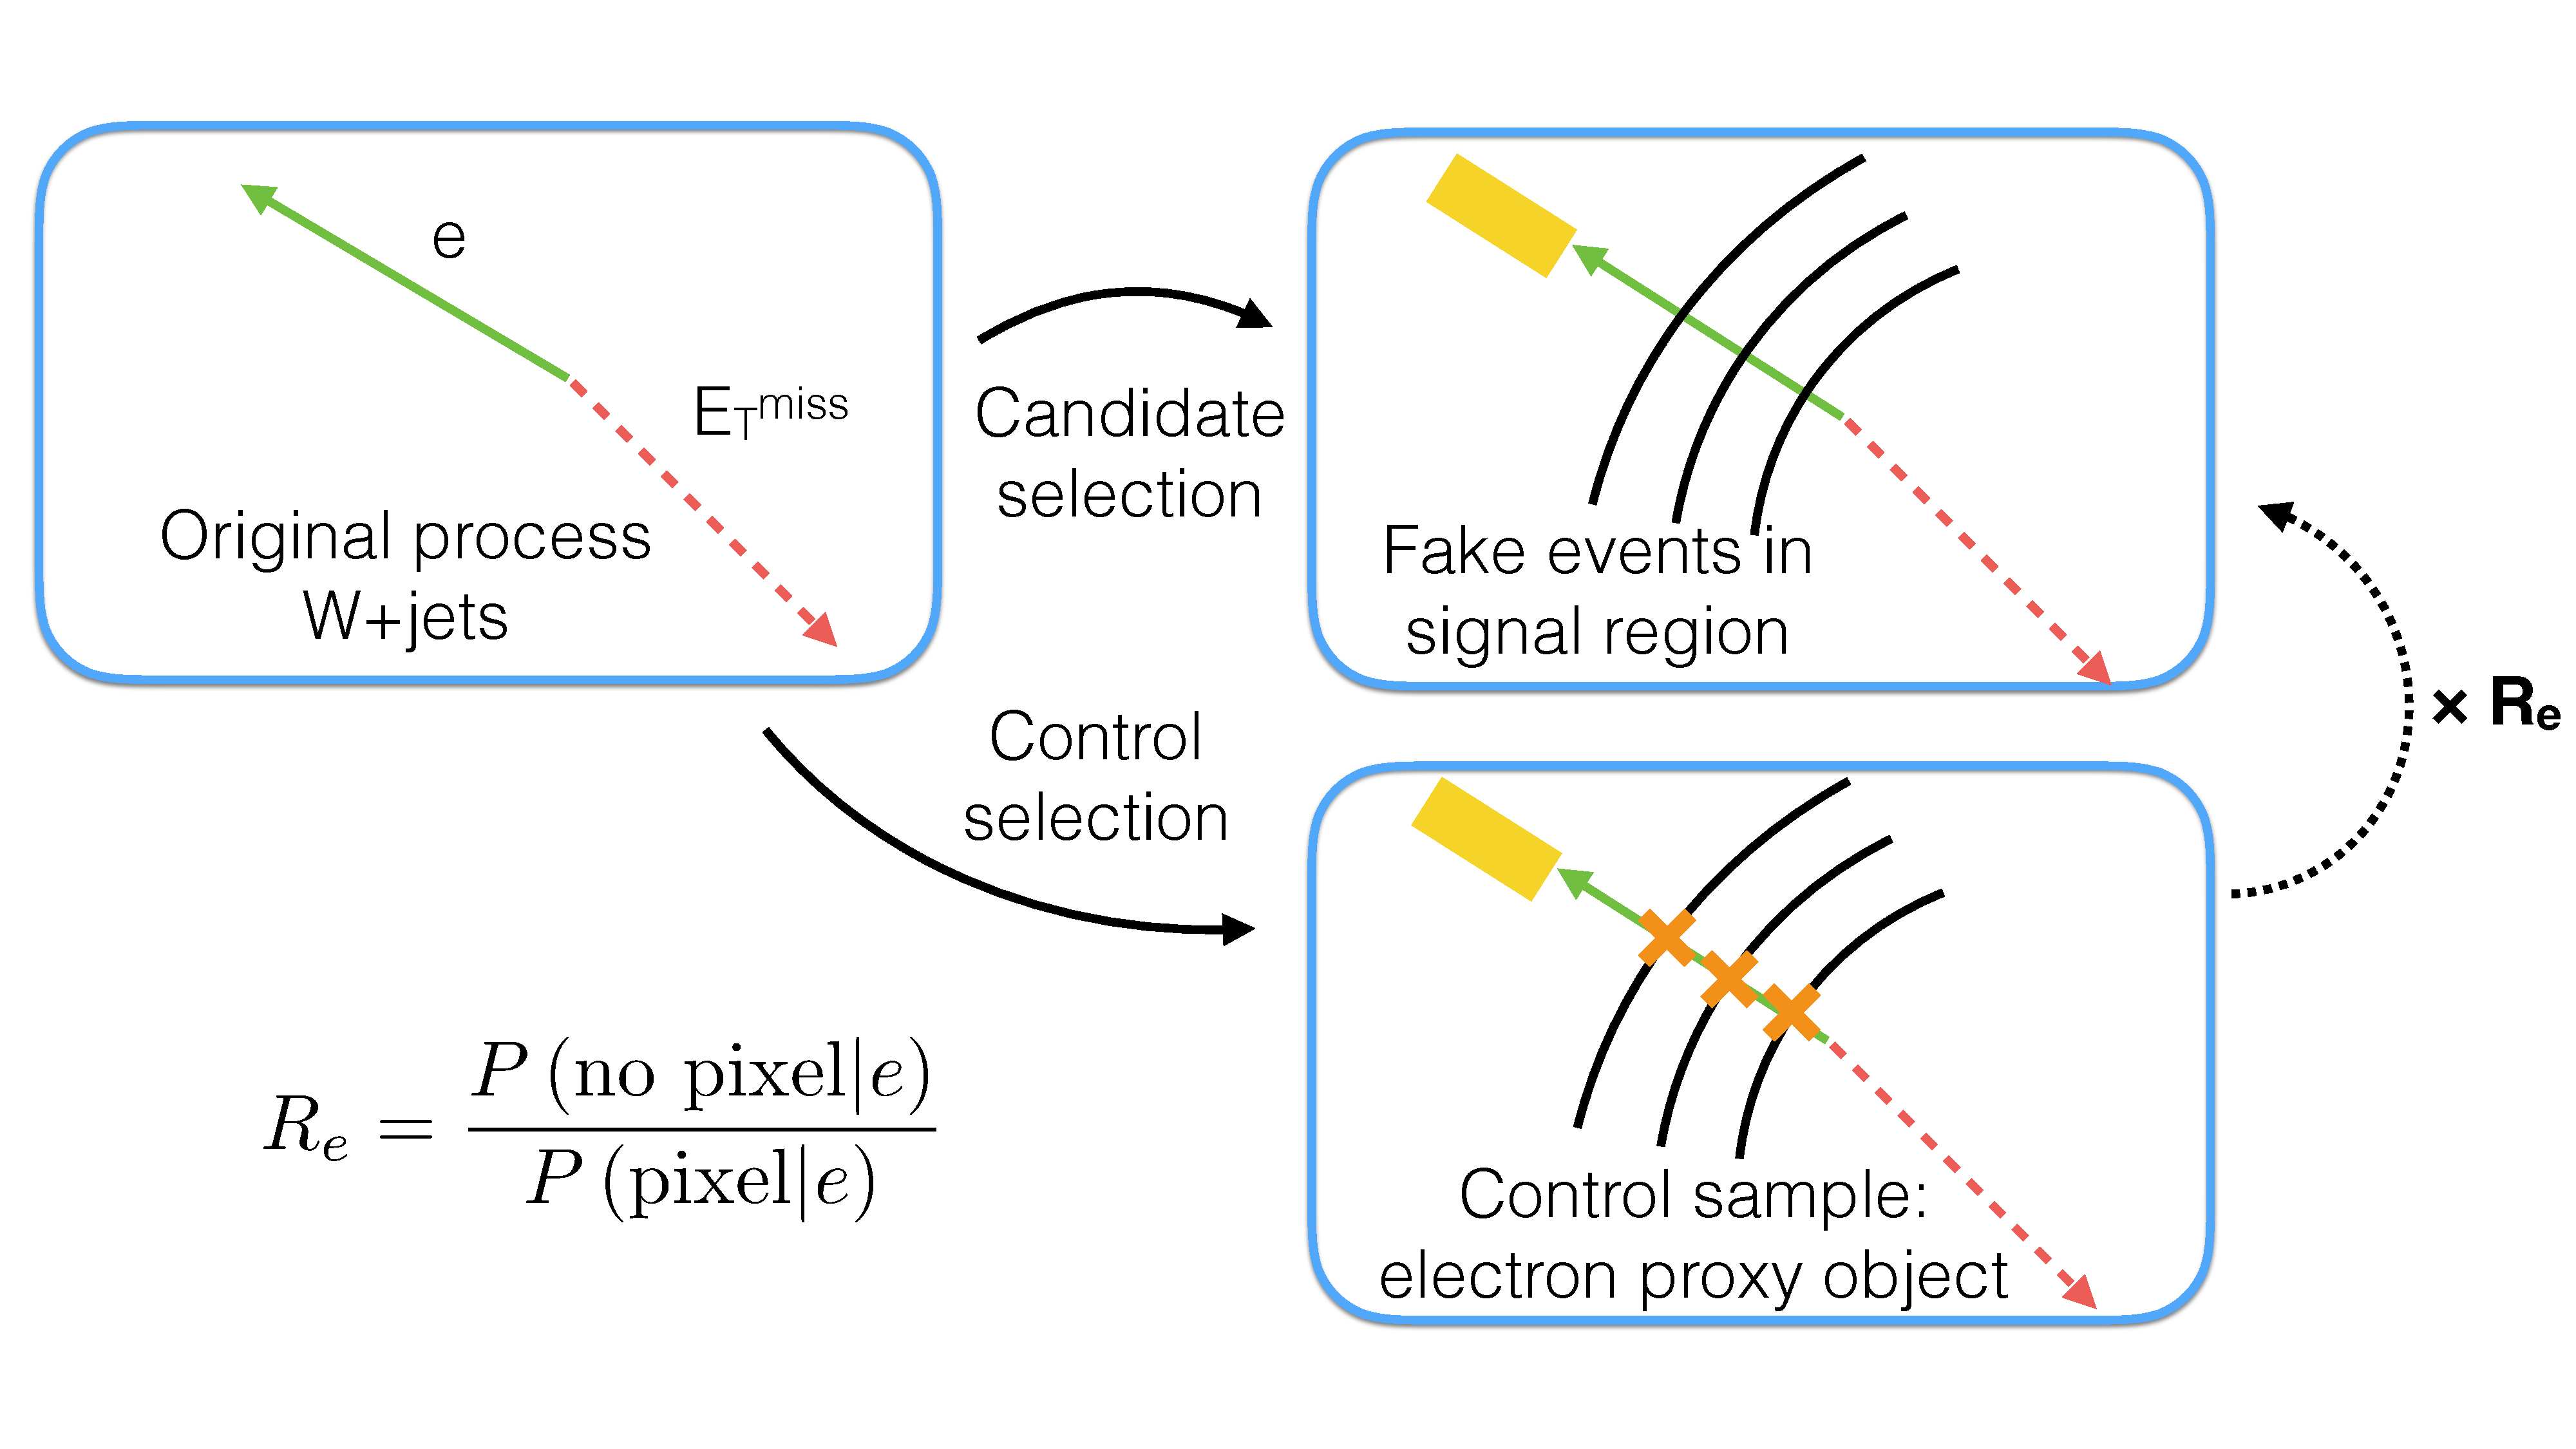
\includegraphics[]{Analysis/Figures/efake/efake_diagram.pdf}
  }
  \caption{
       Events where a single \PW\ boson decays to an electron and a neutrino mimic the photon plus \met\ signature if the electron is missing a pixel seed.
       The rate of misidentified electrons in the signal region is estimated by reweighting an electon proxy control sample by the ratio of the probability of an electron missing a pixel seed to the probability of an electron having a pixel seed.
    }
    \label{fig:efake_diagram}
\end{figure}

The electron-to-photon misidentification rate $R_{\Pe}$ is equal to $(1 - \epsilon_{\Pe}^{\text{track}}) / \epsilon_{\Pe}^{\text{track}}$, where $\epsilon_{\Pe}^{\text{track}}$ is the tracking efficiency of electrons passing the photon identification criteria except for the electron veto.
We measure the factor $R_{\Pe}$ in data using the TP method described in Section~\ref{sec:idsf} with changed definitions for passing and failing probes and an adjustment to the background model.
The \Pe\Pe\ category contains passing probes with a pixel seed while the \Pe\Pgg\ category contains failing probes without a pixel seed.
Probes in both categories must pass the remainder of the \egamma\ and \Pgg-specific IDs.
Denoting the area of the peak in each category $N_{\Pe\Pe}$ and $N_{\Pe\Pgg}$, respectively, the ratio $N_{\Pe\Pgg} / N_{\Pe\Pe}$ is equal to $R_{\Pe}$ up to minor systematic corrections.

Additionally, the backgrounds to the \Pe\Pgg\ fit consist of processes with an electron and an actual photon in the final state, such as \PW\Pgg\ and \Zee\ with a hard radiation off one of the electrons.
To account for the higher rate of bremsstrahlung experienced by electrons than by muons, we scale the mass distribution of the $\Pgm+\Pgg$ sample by the ratio of electron-probe to muon-probe events taken from MC.
As an alternative template to assess the systematic effect introduced by the choice of the background template, the unscaled mass distribution is also tested.

\begin{figure}[htbp]
  \centering
  \resizebox{0.95\textwidth}{!}{
    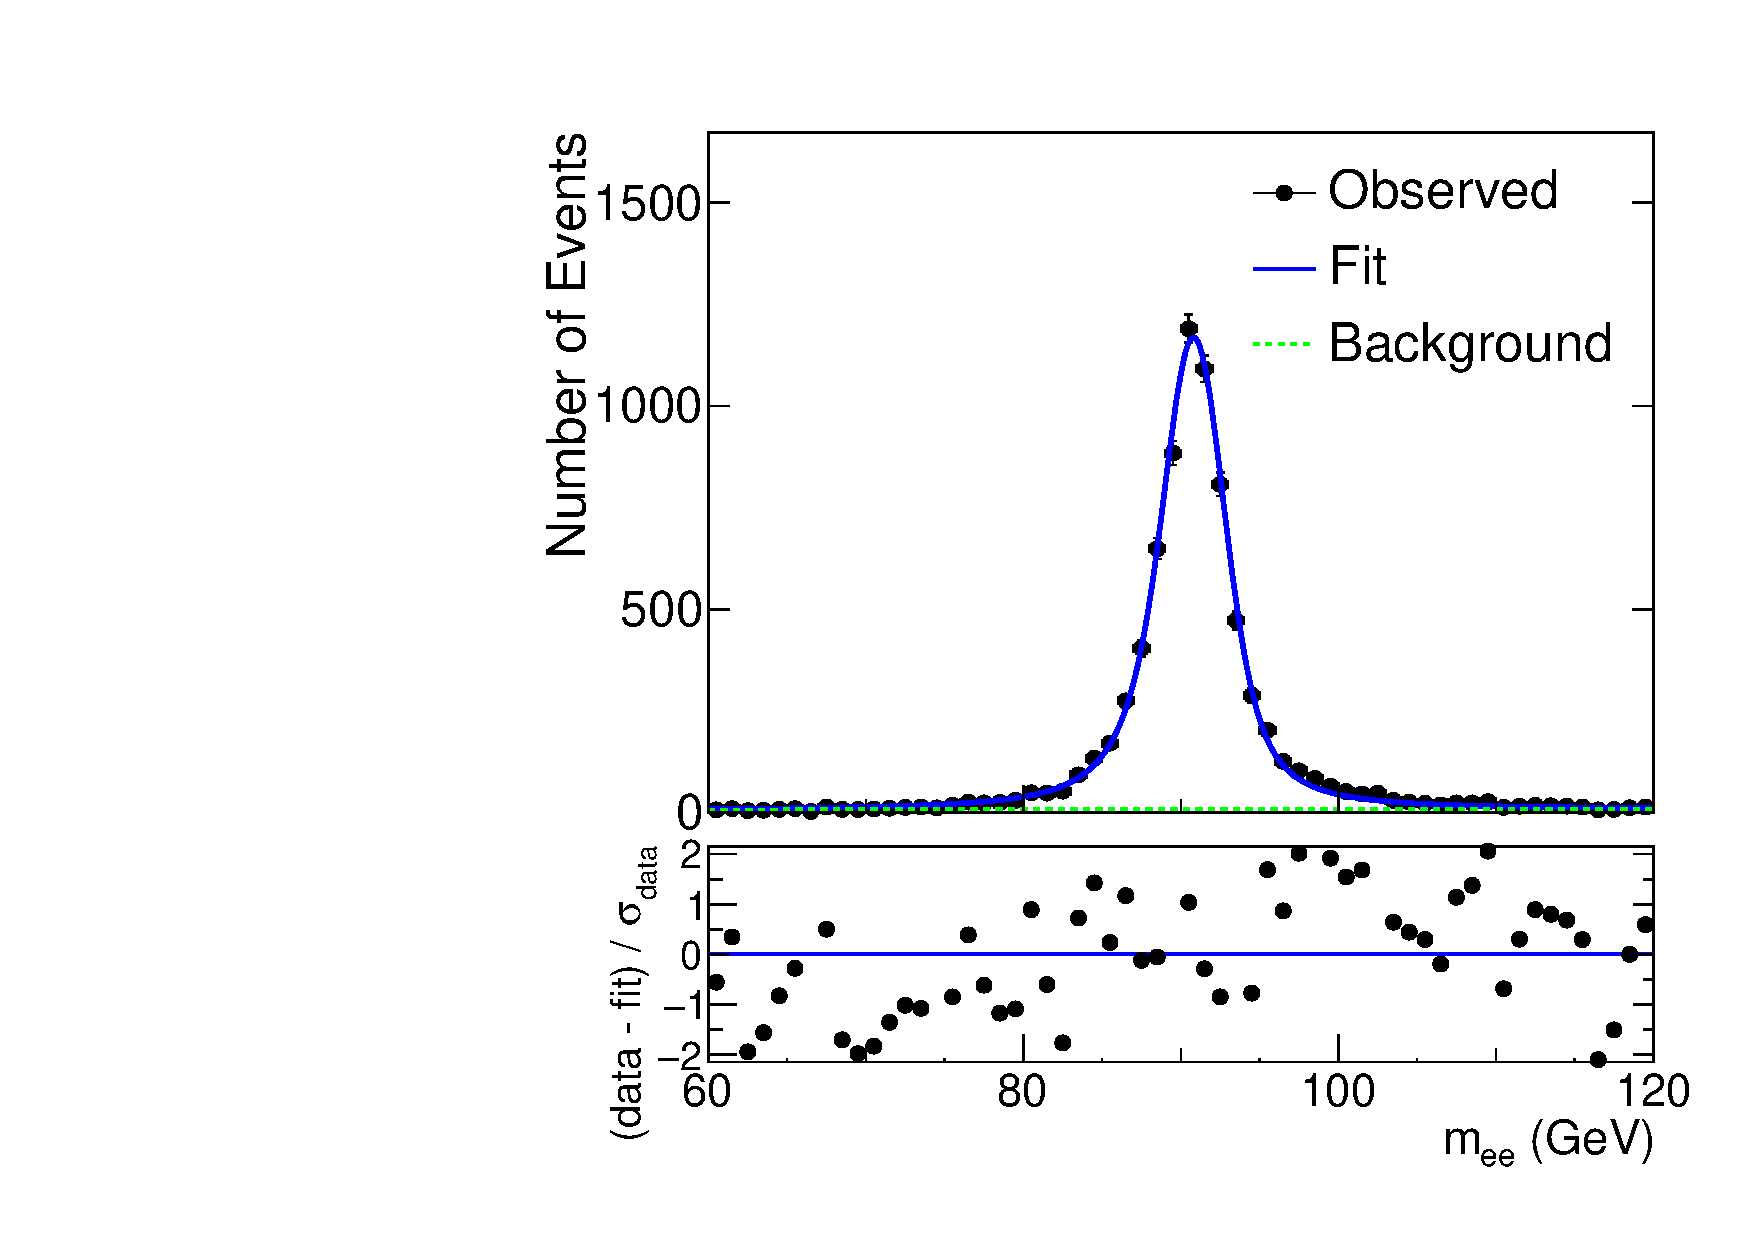
\includegraphics[]{Analysis/Figures/efake/fit_data_ee_pt_175_200.pdf}
    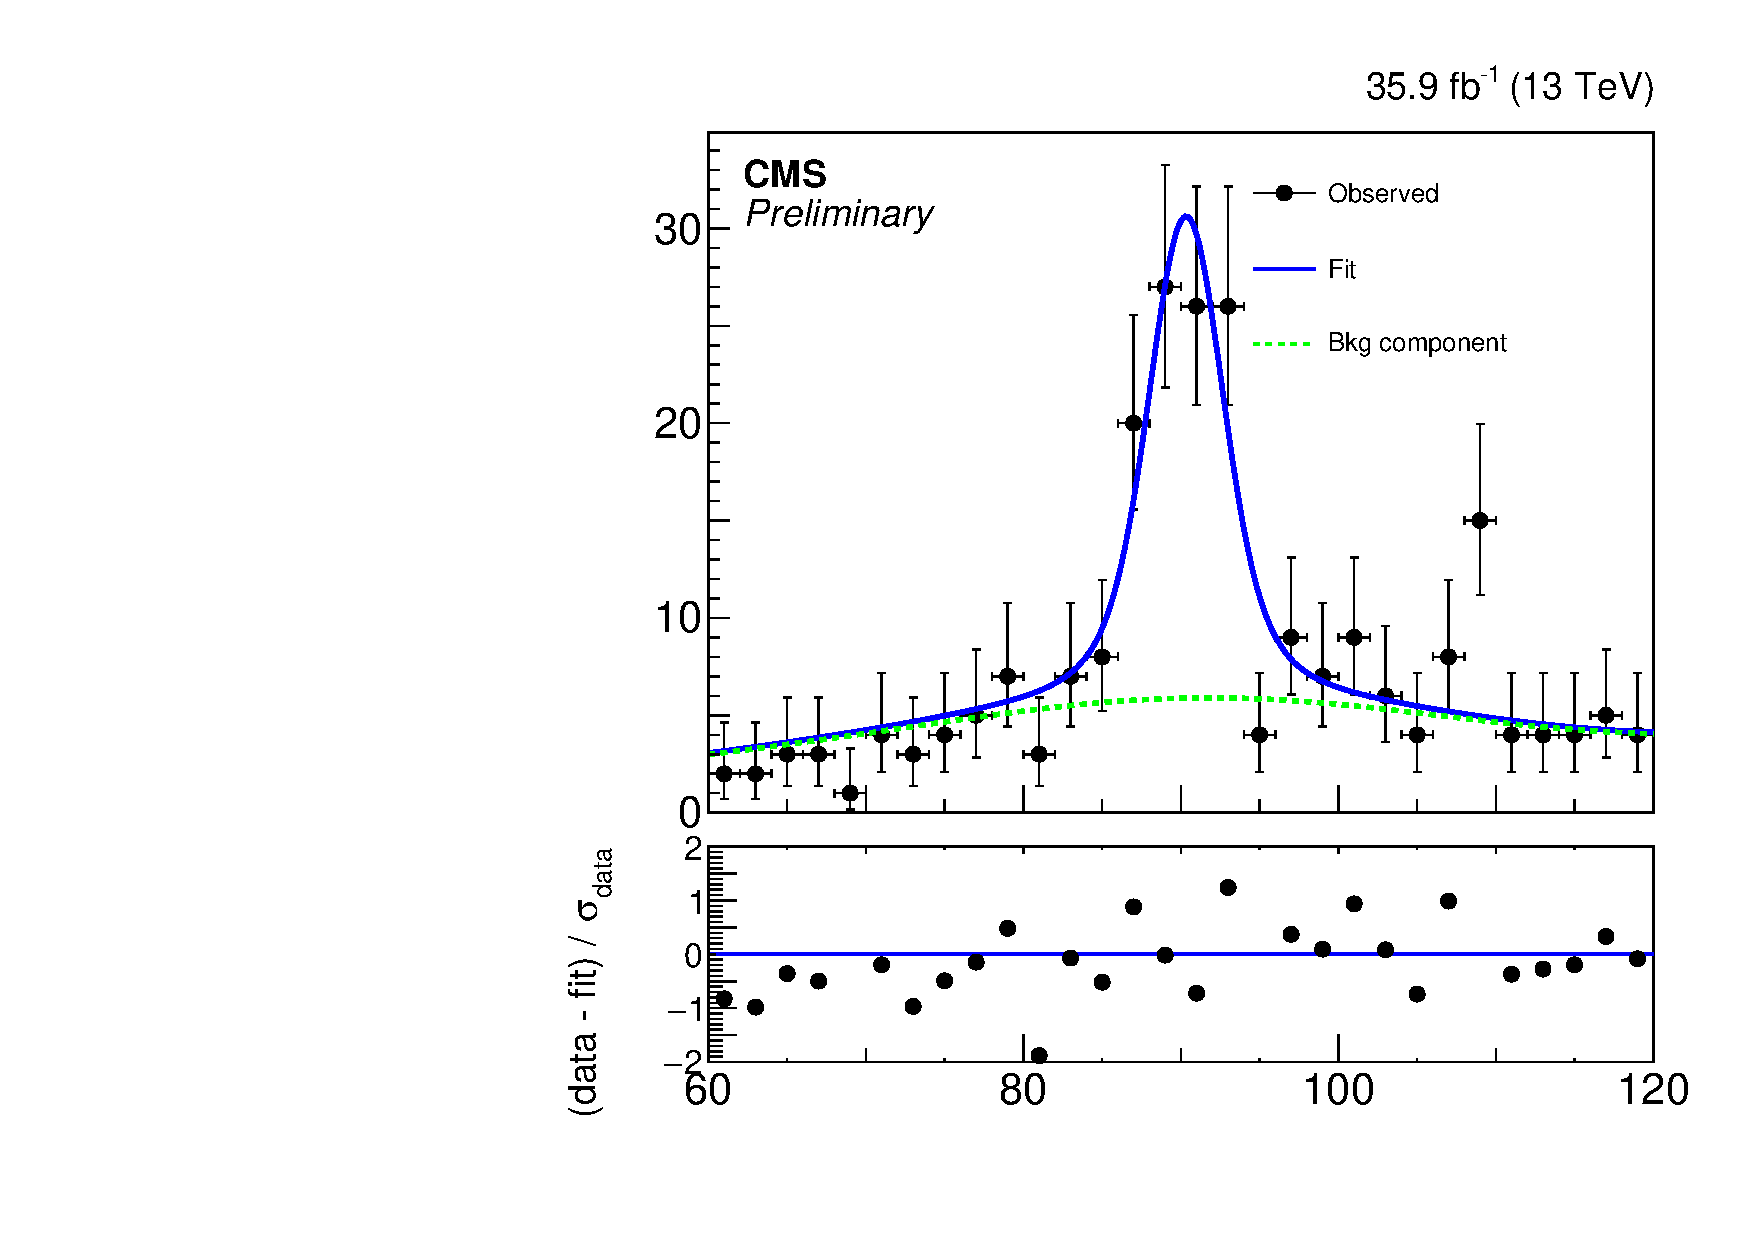
\includegraphics[]{Analysis/Figures/efake/fit_data_eg_pt_175_200.pdf}
  }
  \resizebox{0.95\textwidth}{!}{
    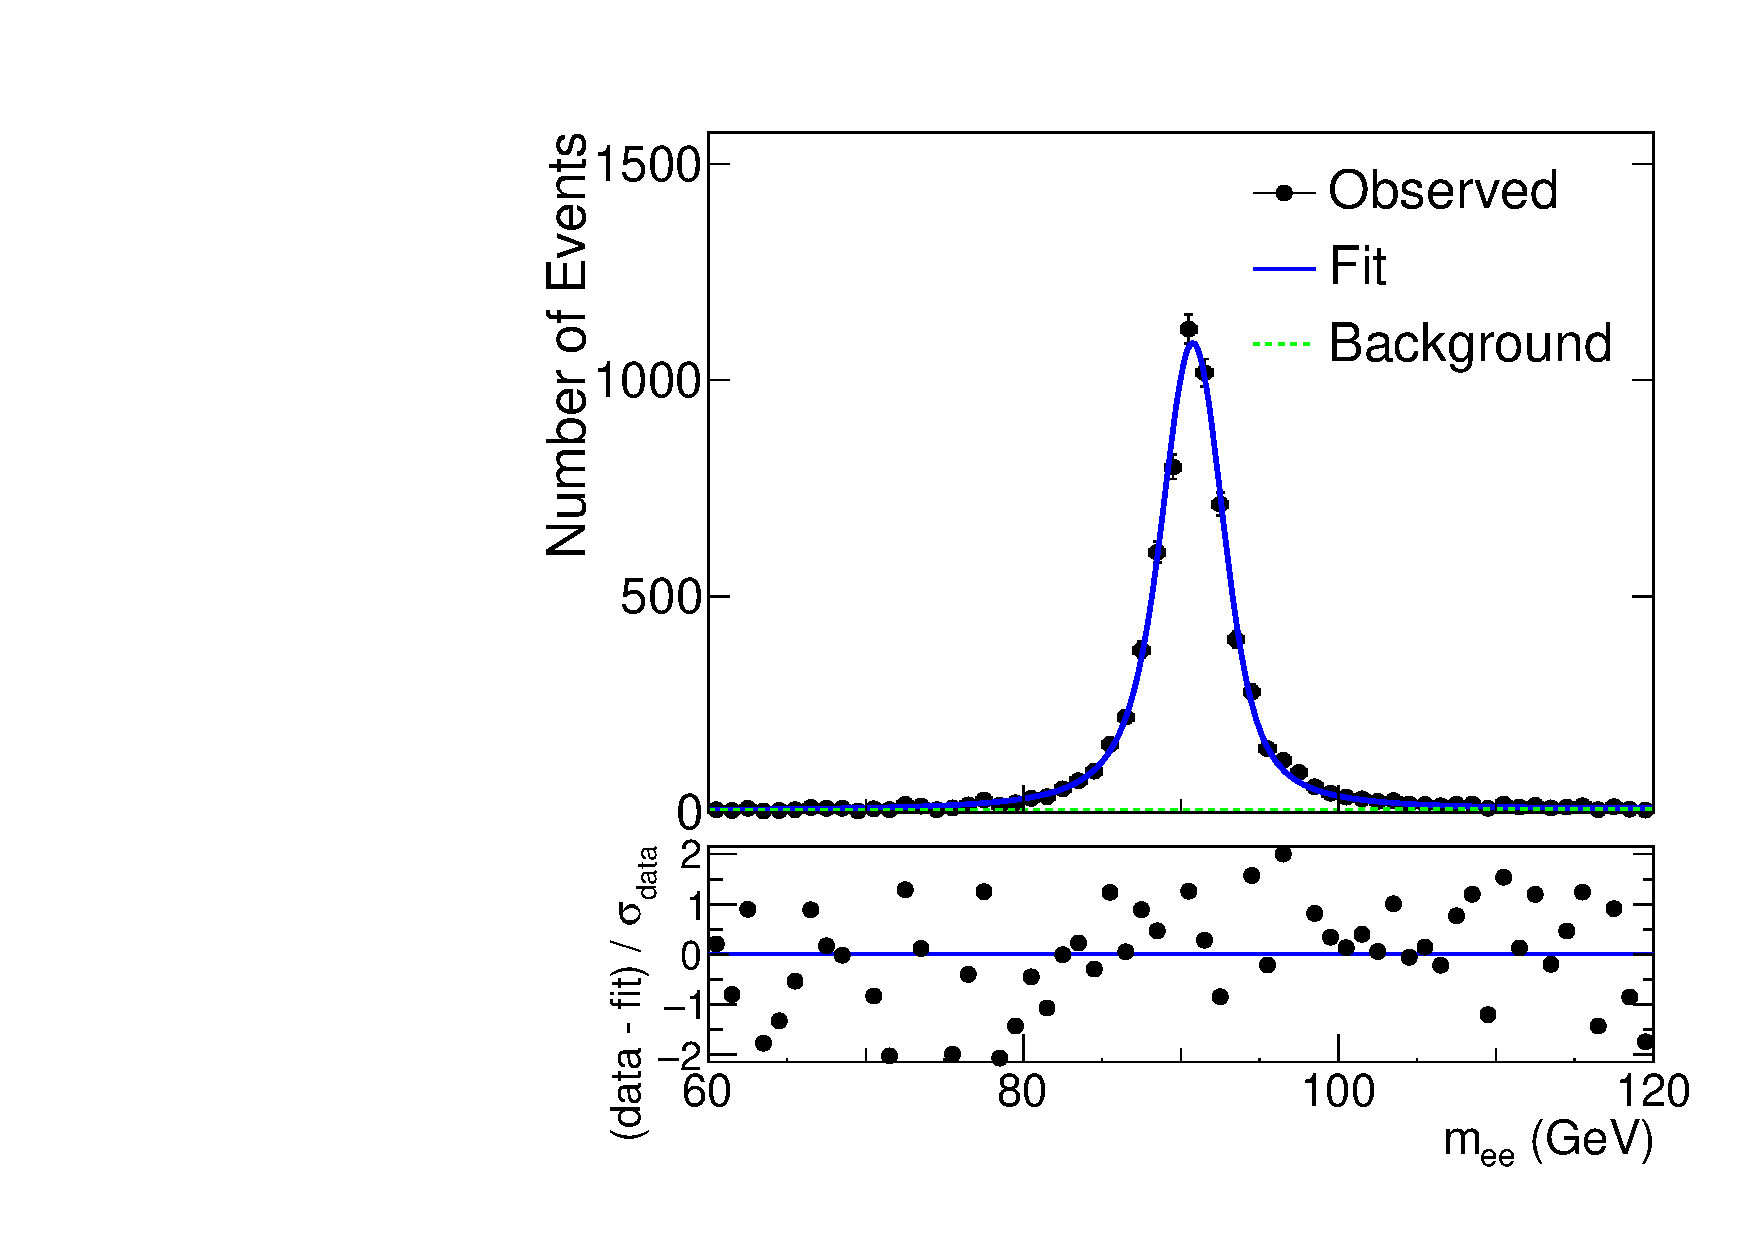
\includegraphics[]{Analysis/Figures/efake/fit_data_ee_pt_200_250.pdf}
    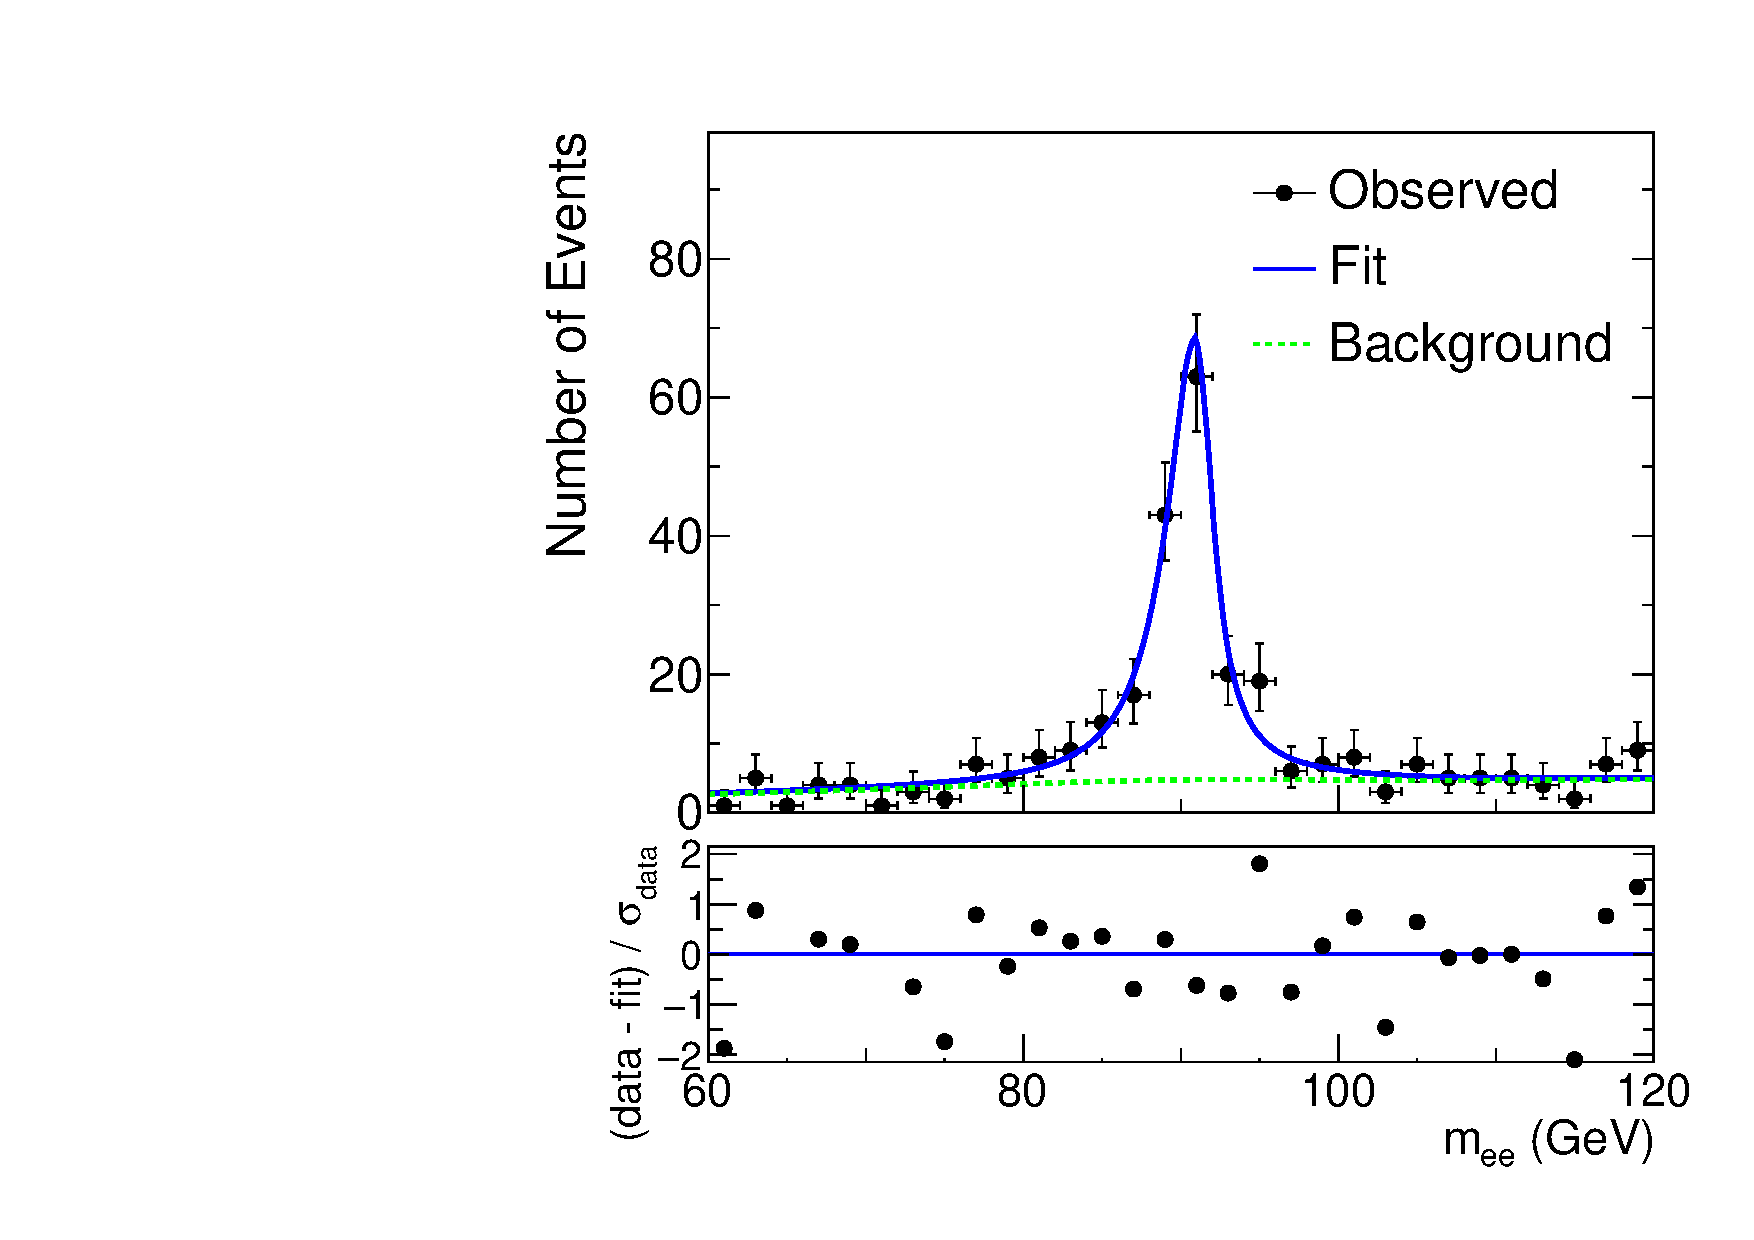
\includegraphics[]{Analysis/Figures/efake/fit_data_eg_pt_200_250.pdf}
  }
  \resizebox{0.95\textwidth}{!}{
    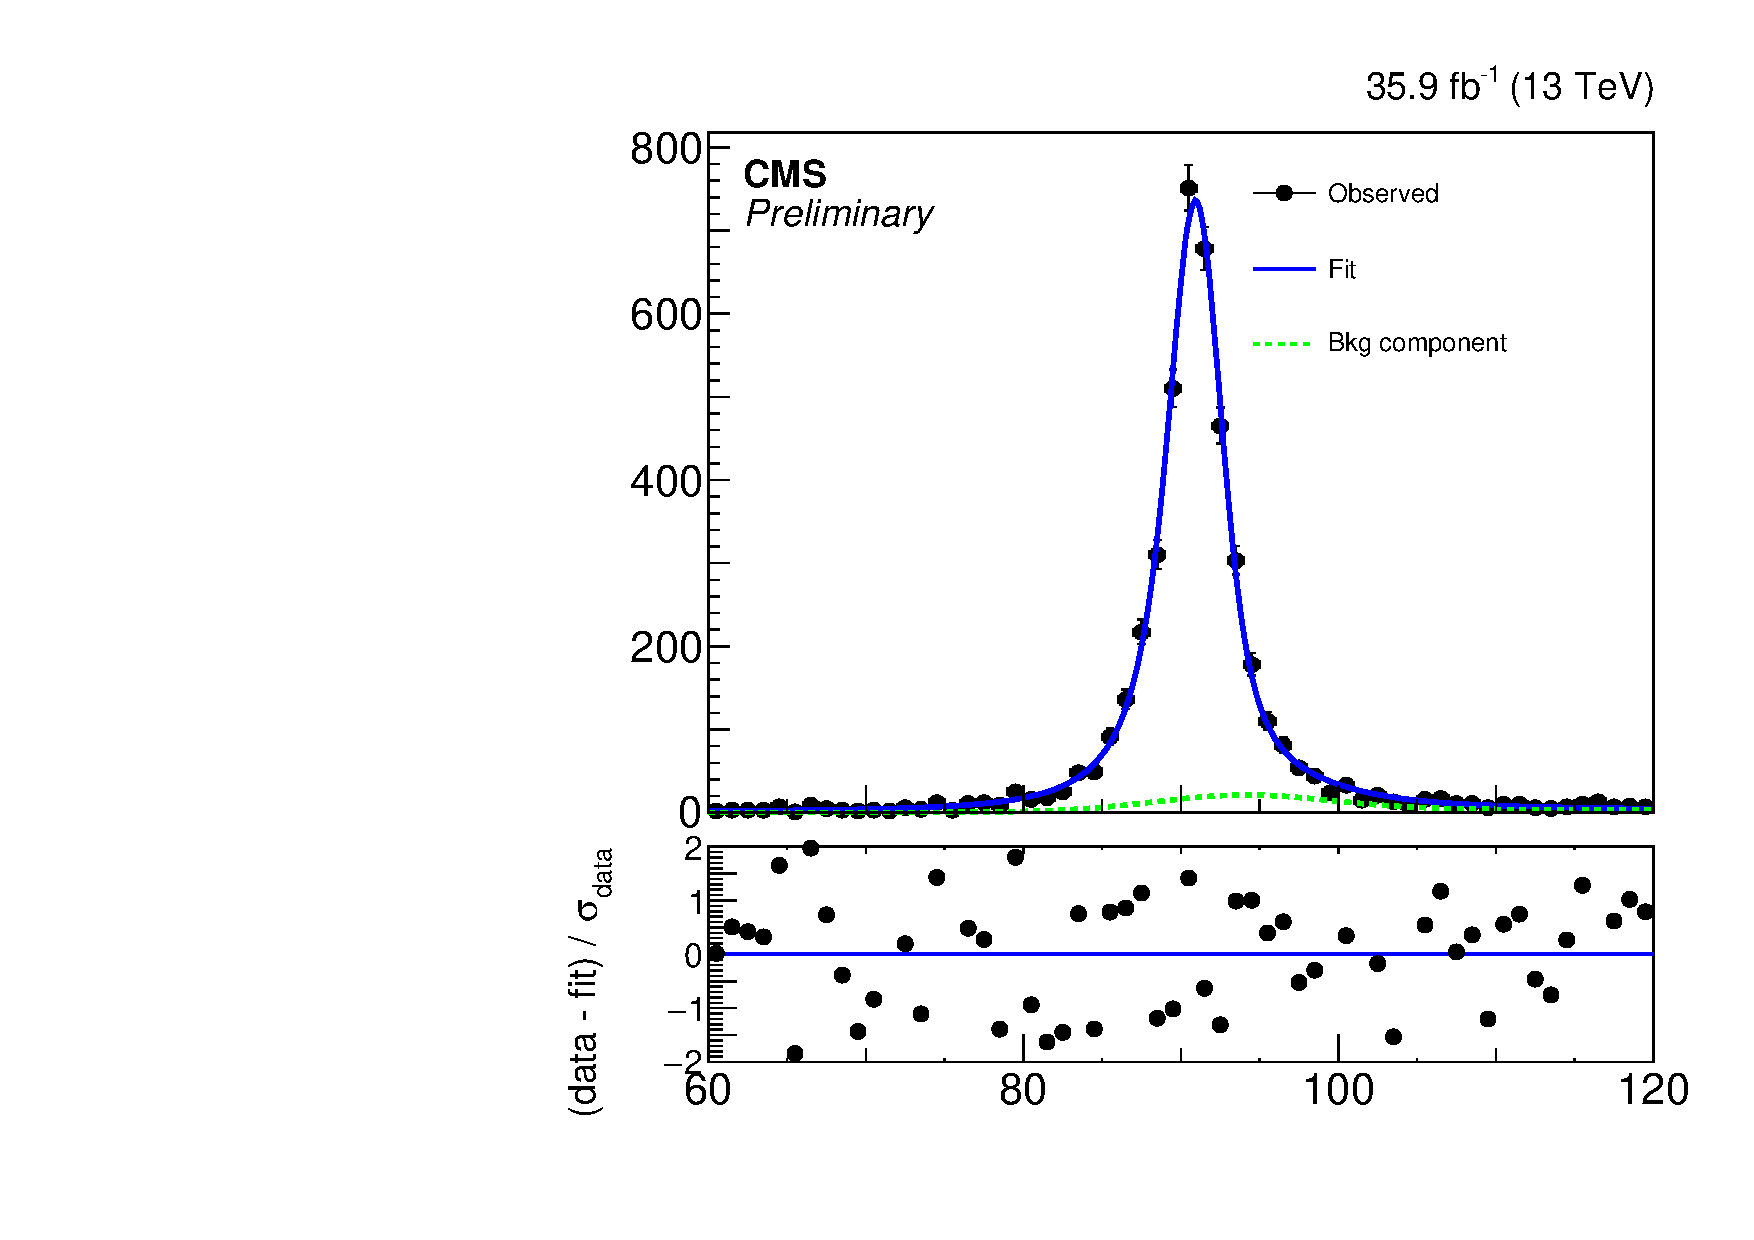
\includegraphics[]{Analysis/Figures/efake/fit_data_ee_pt_250_6500.pdf}
    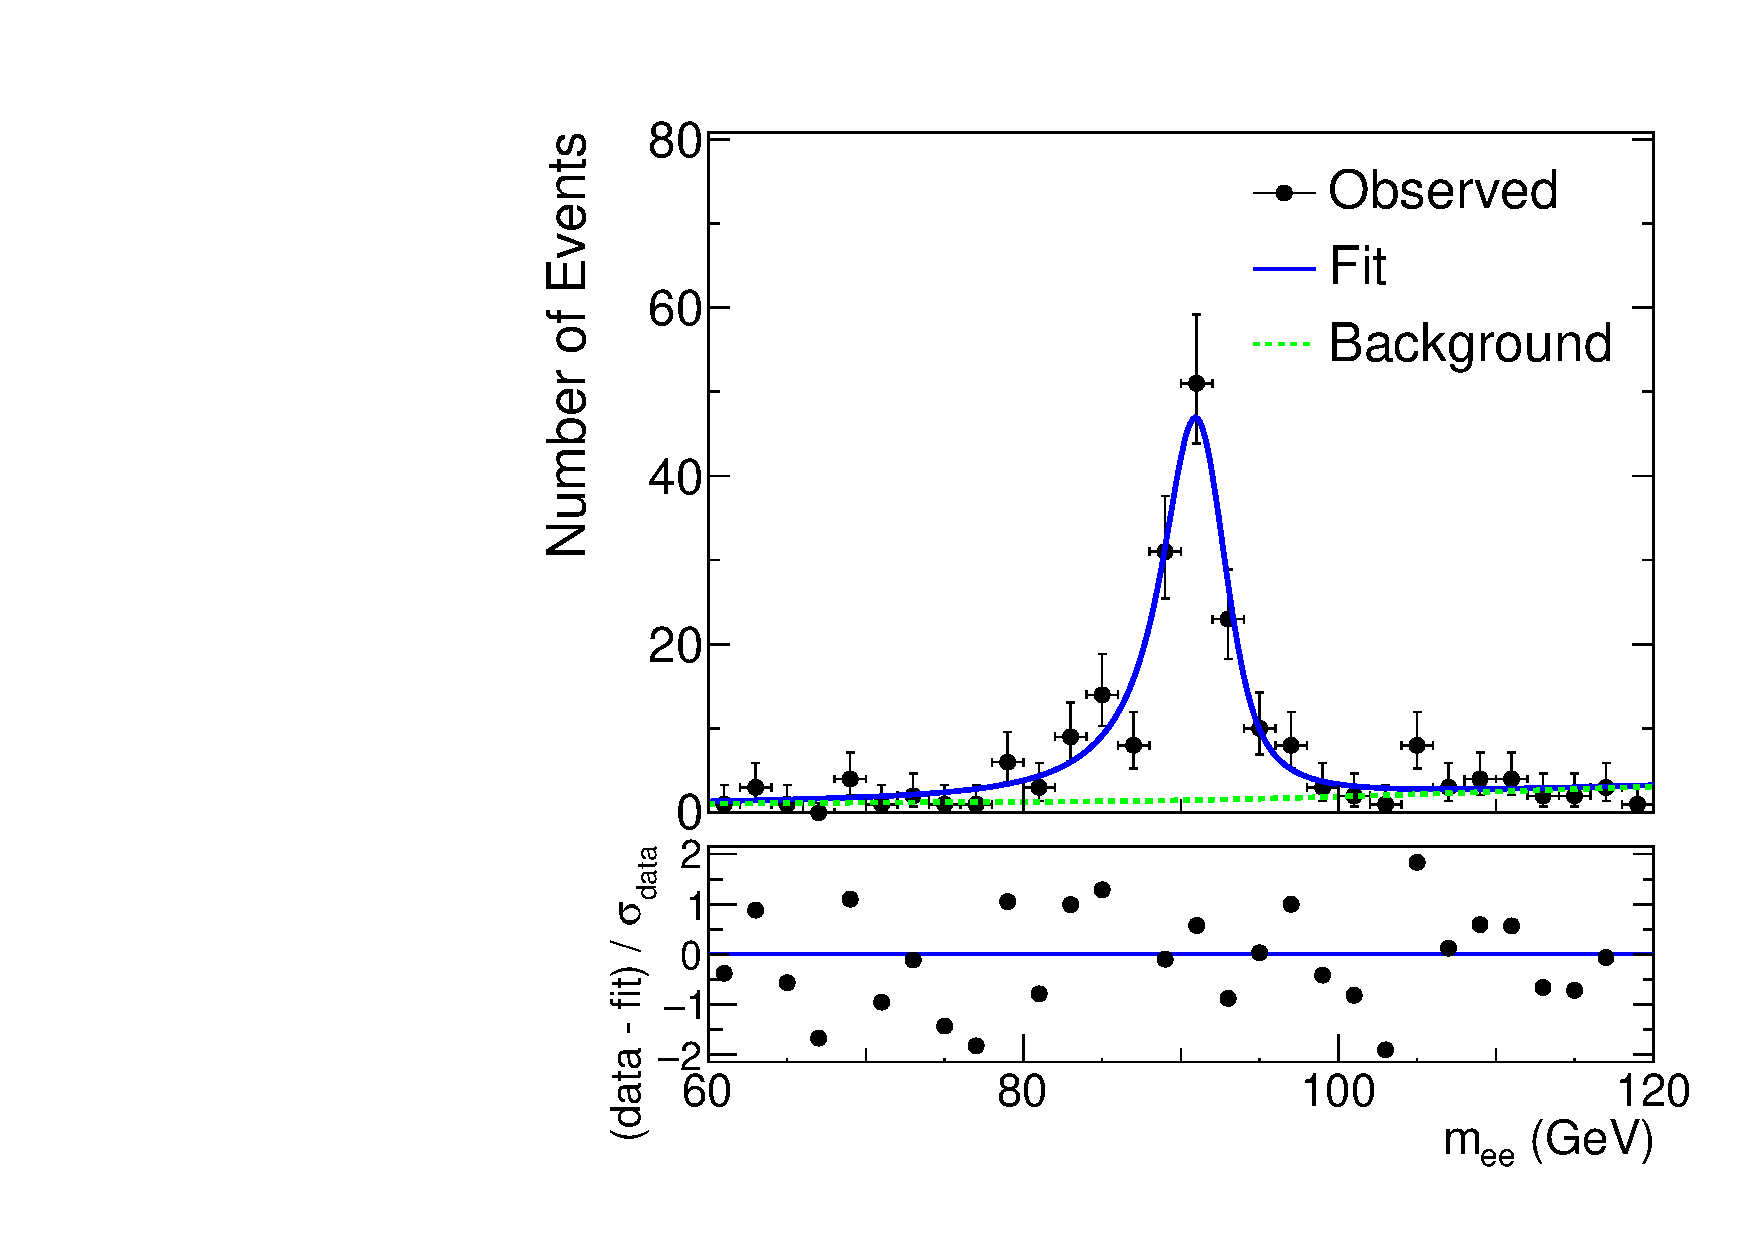
\includegraphics[]{Analysis/Figures/efake/fit_data_eg_pt_250_6500.pdf}
  }
  \caption{
      Fits to the mass distributions for \Pe\Pe\ (left) and \Pe\Pgg\ (right) selections, in bins of probe $\pt$: $175 < \pt < 200\GeV$ (top), $200 < \pt < 250\GeV$ (middle), $\pt > 250\GeV$ (bottom). 
      The blue solid line represents the full fit model, and the green dashed line its background component.
    }
    \label{fig:efake_fits}
\end{figure}

Figure~\ref{fig:efake_fits} shows the six fits performed on \Pe\Pe\ and \Pe\Pgg\ in bins of probe $\pt$, from which the $R_{\Pe}$ factor used for the estimation of the electron misidentification background is derived.
Figure~\ref{fig:efake_frate} shows the derived $R_{\Pe}$ factor as a function of \ETg.

\begin{figure}[htbp]
\centering
    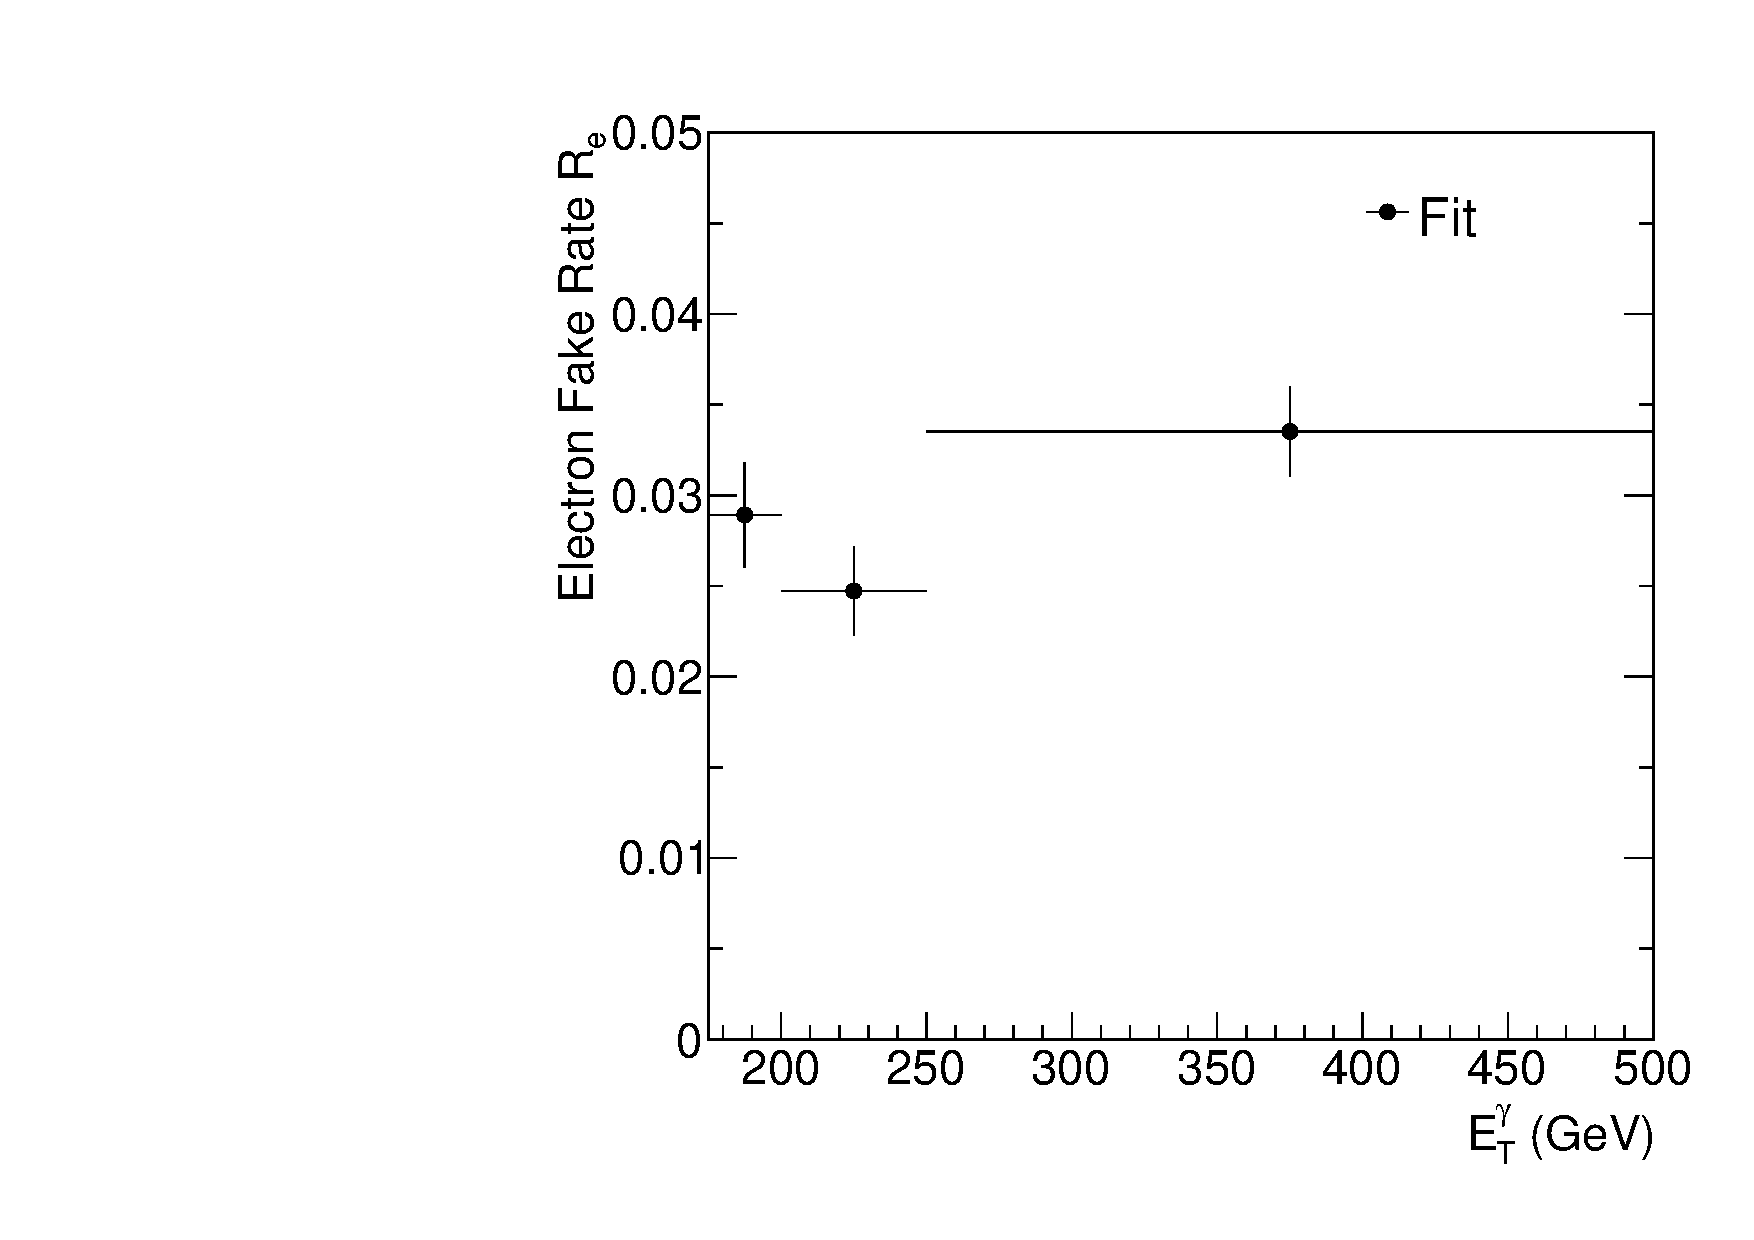
\includegraphics[width=0.5\textwidth]{Analysis/Figures/efake/frate_data_ptalt.pdf} 
    \caption{
      Electron to photon fake rate $R_{\Pe}$.
    }
    \label{fig:efake_frate}
\end{figure}

To estimate the background due to misidentified electrons, an electron proxy+\met\ control sample is used.
This proxy sample is obtained by identical event selection as that of the signal region but with the pixel-seed veto inverted on the photon candidate object.
Such a photon candidate is referred to as a electron proxy object.
This yields a sample of events with similar kinematics to the signal region and well-identified electron candidates, differing only from the misidentified electron events in that a pixel hit was associated with the photon object.
Table~\ref{tab:eleproxy} summarizes the selections for the electron proxy+\met\ control sample. 

\begin{table}[htbp]
  \centering
    \begin{tabular}{l | l | r}
      Variable & Selection & Motivation \\
      \hline
      $\ET$ & $ > 175\GeV$ & electron proxy object passing trigger \\
      $\abs{\eta}$ & $ < 1.44$ & match signal region kinematics \\
      \egamma\ ID & Pass  & must be photon-like \\
      \Pgg-specific ID & Pass non-collision cuts & must be photon-like \\
      Pixel Seed Veto & Fail & inverted to mimic electrons \\
      $\met $ & $ > 170\GeV$ & match signal region kinematics \\
      $\ETg / \met  $ & $ < 1.4$ & match signal region kinematics \\
      $\mindphijmet  $ & $ > 0.5$ & match signal region kinematics \\
      $\dphigmet  $ & $ > 0.5$ & match signal region kinematics \\
      Lepton Veto & Pass & match signal region \\
    \end{tabular}
  \caption{Selections for the electron proxy+\met\ control sample.}
  \label{tab:eleproxy}
\end{table}

After making the reasonable assumption that the kinematic and other critical properties of the electron plus \met\ events are unaffected by the electron misidentification, we model the electron misidentification background by taking the electron proxy+\met\ control sample and reweighting each event by $R_{\Pe}$ depending on the \pt\ of the electron proxy object.
